\documentclass[12pt,a4paper]{article} %437
\usepackage{indentfirst}
\usepackage{amsmath}
\usepackage{enumerate}
\usepackage{amssymb}
\usepackage{graphicx}
\usepackage{color}
\makeatletter
\makeatother
\usepackage[utf8]{inputenc}
\usepackage[T1]{fontenc}
\usepackage{pdflscape}
\usepackage{bm}
\usepackage{float}
%\usepackage[dvips]{graphicx, color}
%\usepackage{subfigure}
%\usepackage[skins,listings,breakable]{tcolorbox}

\usepackage{color}
\definecolor{lbcolor}{rgb}{0.9,0.9,0.9}

%TCIDATA{OutputFilter=latex2.dll}
%TCIDATA{LastRevised=Friday, February 01, 2008 17:54:39}
%TCIDATA{<META NAME="GraphicsSave" CONTENT="32">}


\setlength\topmargin{-1.5cm} \setlength\oddsidemargin{0.0cm}
\setlength\evensidemargin{0.0cm} \setlength{\textwidth}{16cm}
\setlength{\textheight}{25cm}


\newtheorem{definition}{Definition}
\newtheorem{theorem}{Theorem}
\newtheorem{example}{Example}
\newtheorem{corollary}{Corollary}
\newtheorem{lemma}{Lemma}
\newtheorem{proposition}{Proposition}
\newenvironment{proof}{{\bf Proof:\ \ }}{\qed}
\newcommand{\qed}{\rule{0.5em}{1.5ex}}
\newcommand{\bfg}[1]{\mbox{\boldmath $#1$\unboldmath}}
\newcommand{\dse} {\displaystyle}
\newcommand{\real}{{I\!\!R}}
\newcommand{\zern}{{\bf 0}}
\newcommand{\Cn}{{\bf C}}
\newcommand{\dn}{{\bf d}}
\newcommand{\Dn}{{\bf D}}
\newcommand{\Pn}{{\bf P}}
\newcommand{\xn}{{\bf x}}
\newcommand{\Un}{{\bf U}}
\newcommand{\Kn}{{\bf K}}
\newcommand{\Xn}{{\bf X}}
\newcommand{\Vn}{{\bf V}}
\newcommand{\vn}{{\bf v}}
\newcommand{\bn}{{\bf b}}
\newcommand{\an}{{\bf a}}
\newcommand{\cn}{{\bf c}}
\newcommand{\en}{{\bf e}}
\newcommand{\sn}{{\bf s}}
\newcommand{\Bn}{{\bf B}}
\newcommand{\An}{{\bf A}}
\newcommand{\yn}{{\bf y}}
\newcommand{\Yn}{{\bf Y}}
\newcommand{\Zn}{{\bf Z}}
\newcommand{\zn}{{\bf z}}
\newcommand{\Hn}{{\bf H}}
\newcommand{\Gn}{{\bf G}}
\newcommand{\Mn}{{\bf M}}
\newcommand{\fn}{{\bf f}}
\newcommand{\hn}{{\bf h}}
\newcommand{\In}{{\bf I}}
\newcommand{\Fn}{{\bf F}}
\newcommand{\En}{{\bf E}}
\newcommand{\Jn}{{\bf J}}
\newcommand{\Ln}{{\bf L}}
\newcommand{\mn}{{\bf m}}
\newcommand{\rn}{{\bf r}}
\newcommand{\un}{{\bf u}}
\newcommand{\Rn}{{\bf R}}
\newcommand{\Sn}{{\bf S}}
\newcommand{\Tn}{{\bf T}}
\newcommand{\GLn}{{\bf G \bf L}}
\newcommand{\tn}{{\bf t}}
\newcommand{\alpn}{{\mbox{\boldmath $\alpha$}}}
\newcommand{\epsiln}{{\mbox{\boldmath $\epsilon$}}}
\newcommand{\rhn}{{\mbox{\boldmath $\rho$}}}
\newcommand{\betn}{{\mbox{\boldmath $\beta$}}}
\newcommand{\deltn}{{\mbox{\boldmath $\delta$}}}
\newcommand{\sigmn}{{\mbox{\boldmath $\beta$}}}
\newcommand{\gamn}{{\mbox{\boldmath $\gamma$}}}
\newcommand{\Gamn}{{\mbox{\boldmath $\Gamma$}}}
\newcommand{\lamn}{{\mbox{\boldmath $\lambda$}}}
\newcommand{\Lamn}{{\mbox{\boldmath $\Lambda$}}}
\newcommand{\mun}{{\mbox{\boldmath $\mu$}}}
\newcommand{\etn}{{\mbox{\boldmath $\eta$}}}
\newcommand{\tetn}{{\mbox{\boldmath $\theta$}}}
\newcommand{\Tetn}{{\mbox{\boldmath $\Theta$}}}
\newcommand{\Deltn}{{\mbox{\boldmath $\Delta$}}}
\newcommand{\Phin}{{\mbox{\boldmath $\Phi$}}}
\newcommand{\phin}{{\mbox{\boldmath $\phi$}}}
\newcommand{\Psin}{{\mbox{\boldmath $\Psi$}}}
\newcommand{\psin}{{\mbox{\boldmath $\psi$}}}
\newcommand{\Upin}{{\mbox{\boldmath $\Upsilon$}}}
\newcommand{\upin}{{\mbox{\boldmath $\upsilon$}}}
\newcommand{\Sign}{{\mbox{\boldmath $\Sigma$}}}
\newcommand{\Omegn}{{\mbox{\boldmath $\Omega$}}}
\newcommand{\omegn}{{\mbox{\boldmath $\omega$}}}
\newcommand{\eln}{{\mbox{\boldmath $\ell$}}}
\newcommand{\taun}{{\mbox{\boldmath $\tau$}}}

\hyphenation{ge-ne-ra-ted  hy-per-geo-me-tric  cha-rac-te-ri-ze}


\begin{document}

\begin{center}
\section*{\centerline {A new family of distributions: properties and applications}}
\vspace{0.3in}
{\large Gauss M. Cordeiro$^a$ , Maria do Carmo S. Lima$^a$ and Pedro Rafael D. Marinho$^b$}\\
%\vspace{0.3in}
%First Version: 27 July 2010\\
%\vspace{0.1in}
%This Version: 27 January 2011\\
\end{center}

\begin{abstract}\noindent
This article introduces a new family by combining the Marshall and Olkin-G and Gamma-G classes. The family has only two
extra shape parameters and can be a better alternative than other existing classes of distributions. Simulations are performed to verify the
consistency of the estimators. Its flexibility is shown using two real data sets.
\end{abstract}

\vspace{0.5in}
\noindent {\bf Key Words}: \\ \\
%\noindent {\bf JEL Codes}: C16, G1 \\ \\
\noindent $^{a}$  Department of Statistics, Federal University of Pernambuco, Recife, Brazil.\\
\noindent $^{b}$ Department of Statistics, Federal University of Paraíba, João Pessoa, Brazil.\\
E-mail:\emph{gausscordeiro@de.ufpe.br, maria@de.ufpe.br, pedro.rafael.marinho@gmail.com} \\


\section{Introduction}

The mechanism by adding shape parameters to a baseline distribution has
proved to be useful to make the generated distributions more flexible especially for studying tail
properties than existing distributions and for improving their goodness-of-fit statistics
to the data under study.

Let $G(x)$ be the cumulative distribution function (CDF) of a
baseline distribution and $g(x)=dG(x)/dx$ be the corresponding  probability density function (PDF) depending on a
parameter vectot $\eta$. A generalized family are presented
with two additional shape parameters by transforming the CDF $G(x)$
according to two sequential important gene\-rators. These families are important for modeling data
in several engineering areas. Many special distributions in these families are discussed by Tahir
and Nadarajah (2015).


The CDF of the Marshall and Olkin's (1997) ($\text{MO-G}$) family (for $\theta>0$) is
\begin{equation}\label{CDF_MO}
F_{\text{MO-G}}(x)=\frac{G(x)}{\theta+(1-\theta)G(x)}=\frac{G(x)}{1-(1-\theta)[1-G(x)]},\quad x \in \mathbb{R}.
\end{equation}

The density function corresponding to (\ref{CDF_MO}) has the form
\begin{equation}\label{densityMO}
f_{\text{MO-G}}(x)=\frac{\theta\, g(x)}{[\theta+(1-\theta)G(x)]^{2}}.
\end{equation}

For $\theta=1$, $f_{\text{MO-G}}(x)$ is equal to $g(x)$.
Equation \eqref{densityMO} represents the PDF of the minimum of $n$ iid random variables having density $g(x)$, say $T_1,\cdots,T_N$,
where $N$ has a geometric distribution with probability parameters $\theta$ and $\theta^{-1}$ if $0<\theta<1$ and $\theta>1$,
respectively.

Tahir and Nadarajah (2015, Table 2) presented thirty distributions
belonging to this family. It is easily generated from the baseline quantile function (QF) by
$Q_{\text{MO-G}}(u)=Q_{G}\left(\theta u \left[\theta u+1-u\right]\right)$ for $u\in(0,1)$.

Marshall and Olkin considered the exponential and Weibull distributions for the baseline G and derived some
structural properties of the generated distributions. The special case that G is an exponential distribution
refers to a two-parameter competitive model to the Weibull and gamma distributions.

The CDF of the gamma-G ($\Gamma$-G) family (Zografos and Balakrishnan, 2009) is
\begin{eqnarray}\label{CDF_Ga}
F_{\Gamma\text{-G}}(x)=\gamma_1\left( a, -\log \left[1-G(x)\right]\right), \quad x \in \mathbb{R},
\end{eqnarray}
where $a>0$ is an extra shape parameter,  $\gamma_1(a,z)= \gamma(a,z)/\Gamma(a)$ is the incomplete gamma function ratio
and $\gamma(a,z)=\int_0^{z} t^{a-1}\,\rm{e}^{-t}dt$.

Then, the PDF of the $\Gamma$-G family can be expressed as
\begin{eqnarray}\label{PDF_Ga}
\displaystyle
f_{\Gamma\text{-G}}(x)=\frac{\displaystyle 1}{\displaystyle \Gamma(a)} \left\{ -\log[1-G(x)] \right\}^{a-1}\, g(x).
\end{eqnarray}

Each new $\Gamma$-G distribution follows from a given baseline G.
For $a=1$, the $\Gamma$-G family reduces to G.
If $Z$ is a gamma random variable with unit scale
parameter and shape parameter $a>0$, then $W=Q_G(1-\rm{e}^{Z})$ has density (\ref{PDF_Ga}). So,
the $\Gamma$-G distribution is easily generated from the gamma distribution and the QF of G.




The remaining of the paper is addressed as follows. Section \ref{sec:MOGaG} introduces the {\it Marshall and Olkin-Gamma-G} (MO-$\Gamma$-G)
family and presents some special models. The maximum likelihood estimates (MLEs) of the parameters of the new family is addressed
in Section \ref{estimation}. Some simulations ate performed in Section \ref{sec:simulation} to estimate the biases of the MLEs. Two
empirical applications illustrate the potentiality of the proposed family in Section \ref{applications}. A variety of theoretical properties are derived
in Section \ref{properties}. Some conclusions remarks are offered in Section \ref{conclusions}.


\section{The New Family}\label{sec:MOGaG}


By combining Equations (\ref{CDF_MO}) and (\ref{CDF_Ga}), the CDF of the random variable $X\sim$MO-$\Gamma$-G
representing the new family is defined by
\begin{equation}\label{CDF_MO-Gamma-G}
F_{X}(x)=\frac{\gamma_1\left( a, -\log \left[1-G(x)\right]\right)}{\theta+(1-\theta)\gamma_1\left( a, -\log \left[1-G(x)\right]\right)},\quad x \in \mathbb{R}.
\end{equation}

By differentiating (\ref{CDF_MO-Gamma-G}), the PDF of $X$ follows as
\begin{equation}\label{PDF_MO-Gamma-G}
f_{X}(x)=\frac{\theta  \left\{ -\log[1-G(x)] \right\}^{a-1}\, g(x)}{\Gamma(a)\,\left\{\theta+(1-\theta)\gamma_1\left( a, -\log \left[1-G(x)\right]\right)\right\}^{2}}.
\end{equation}

The density (\ref{PDF_MO-Gamma-G}) can be interpreted from a sequence of $N$ iid random variables, say $Z_1,\cdots,Z_N$,
each one having a gamma density unit scale and shape $a>0$, assuming that $N$ (is not fixed) has a geometric
distribution with probabilities $\theta$ and $\theta^{-1}$ for $0<\theta<1$ and $\theta>1$,
respectively. By transforming the $Z_i$'s via the baseline QF by $W_i=Q_G(1-\rm{e}^{Z_i})$
(for $i-1,\ldots,N$), Equation \eqref{densityMO} is defined the PDF of the minimum $W_1,\cdots,W_n$.
Making this double composition of the two generators, the proposed family absorbs the impacts of two different flexibilities
on applications.


Table \ref{tabspecial1} provides some special cases of (\ref{PDF_MO-Gamma-G}), where
$\Phi(x)$ and $\phi(x)$ are the CDF and PDF of the standard normal distribution. The density and hazard functions
of the Marshall-Olkin-$\Gamma$-Weibull (MO-$\Gamma$-W) are displayed in Figure \ref{formas}, which provide
more flexibility for these functions in relation to the baseline ones.

%\begin{figure}[h!]
%\begin{center}
%(a)\hspace{3.5cm} (b)\\
%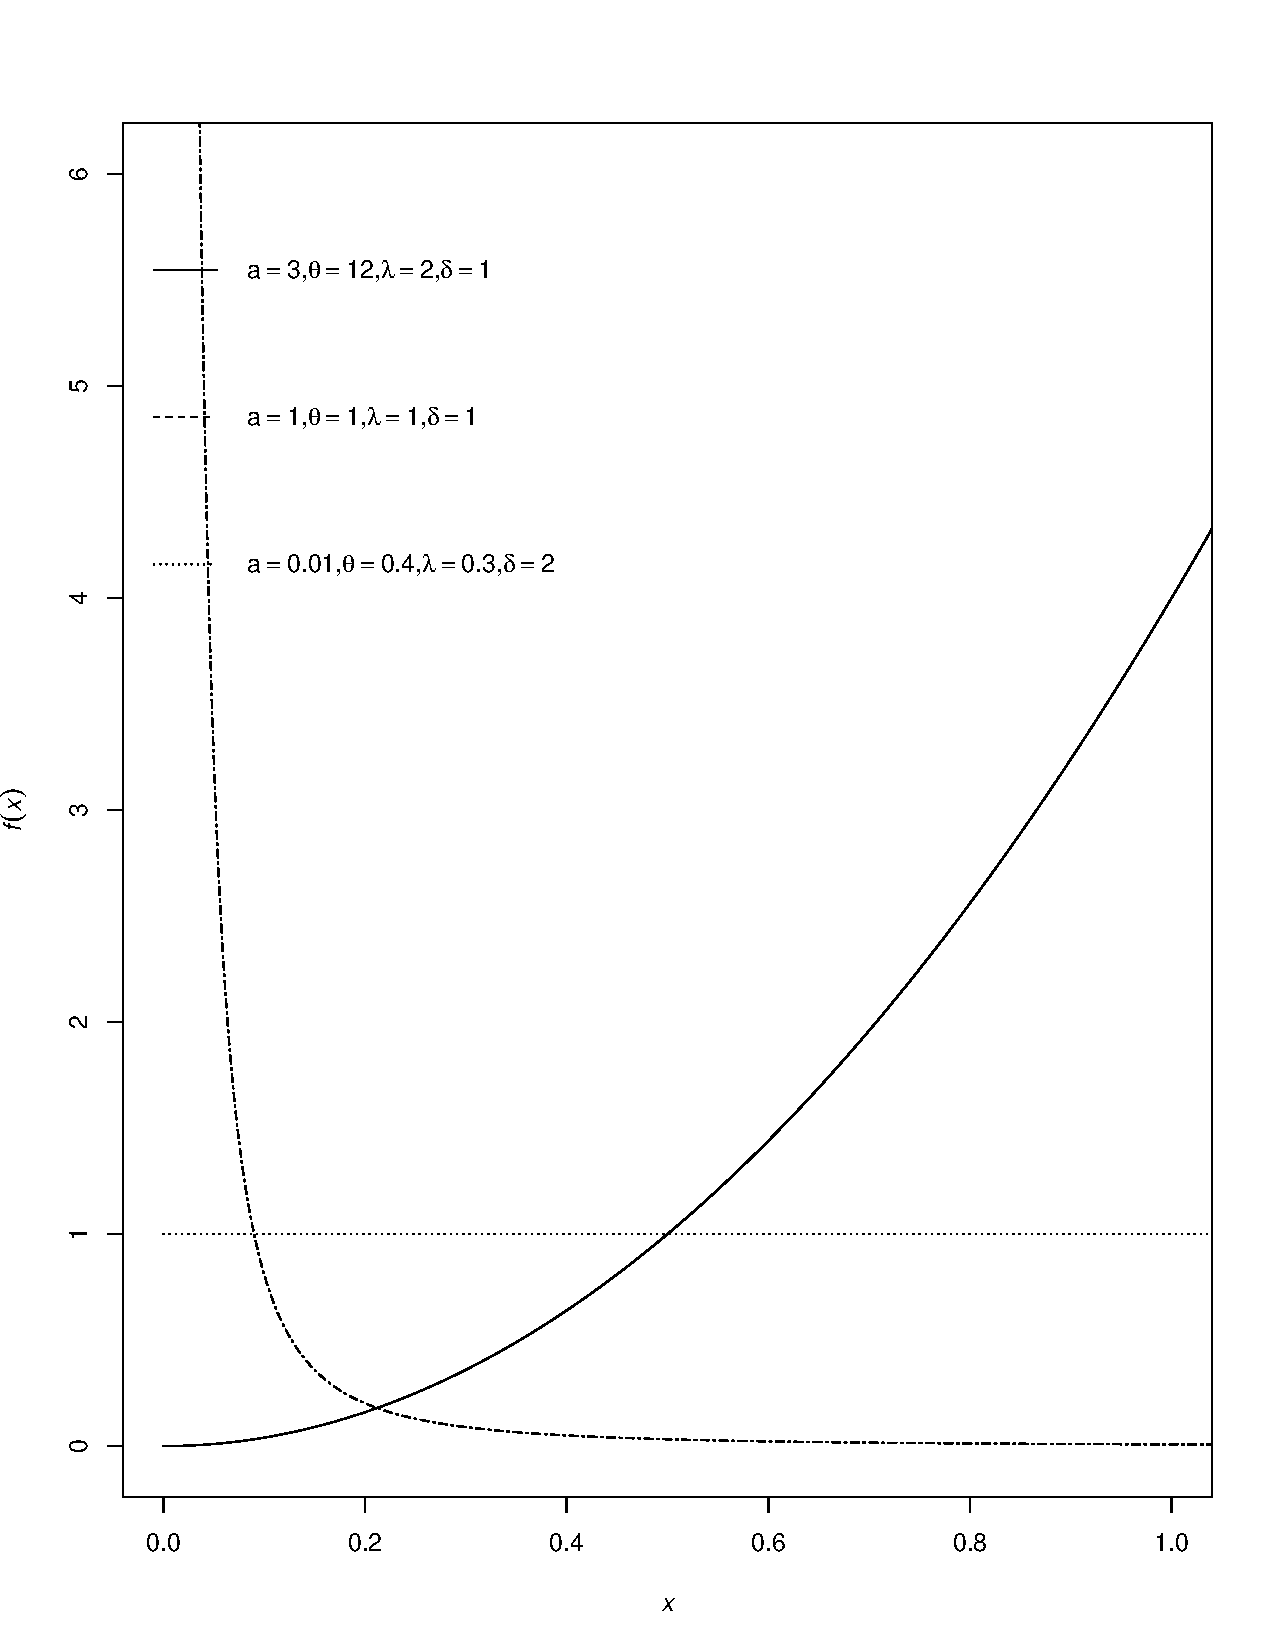
\includegraphics[scale=.3]{density.pdf}
%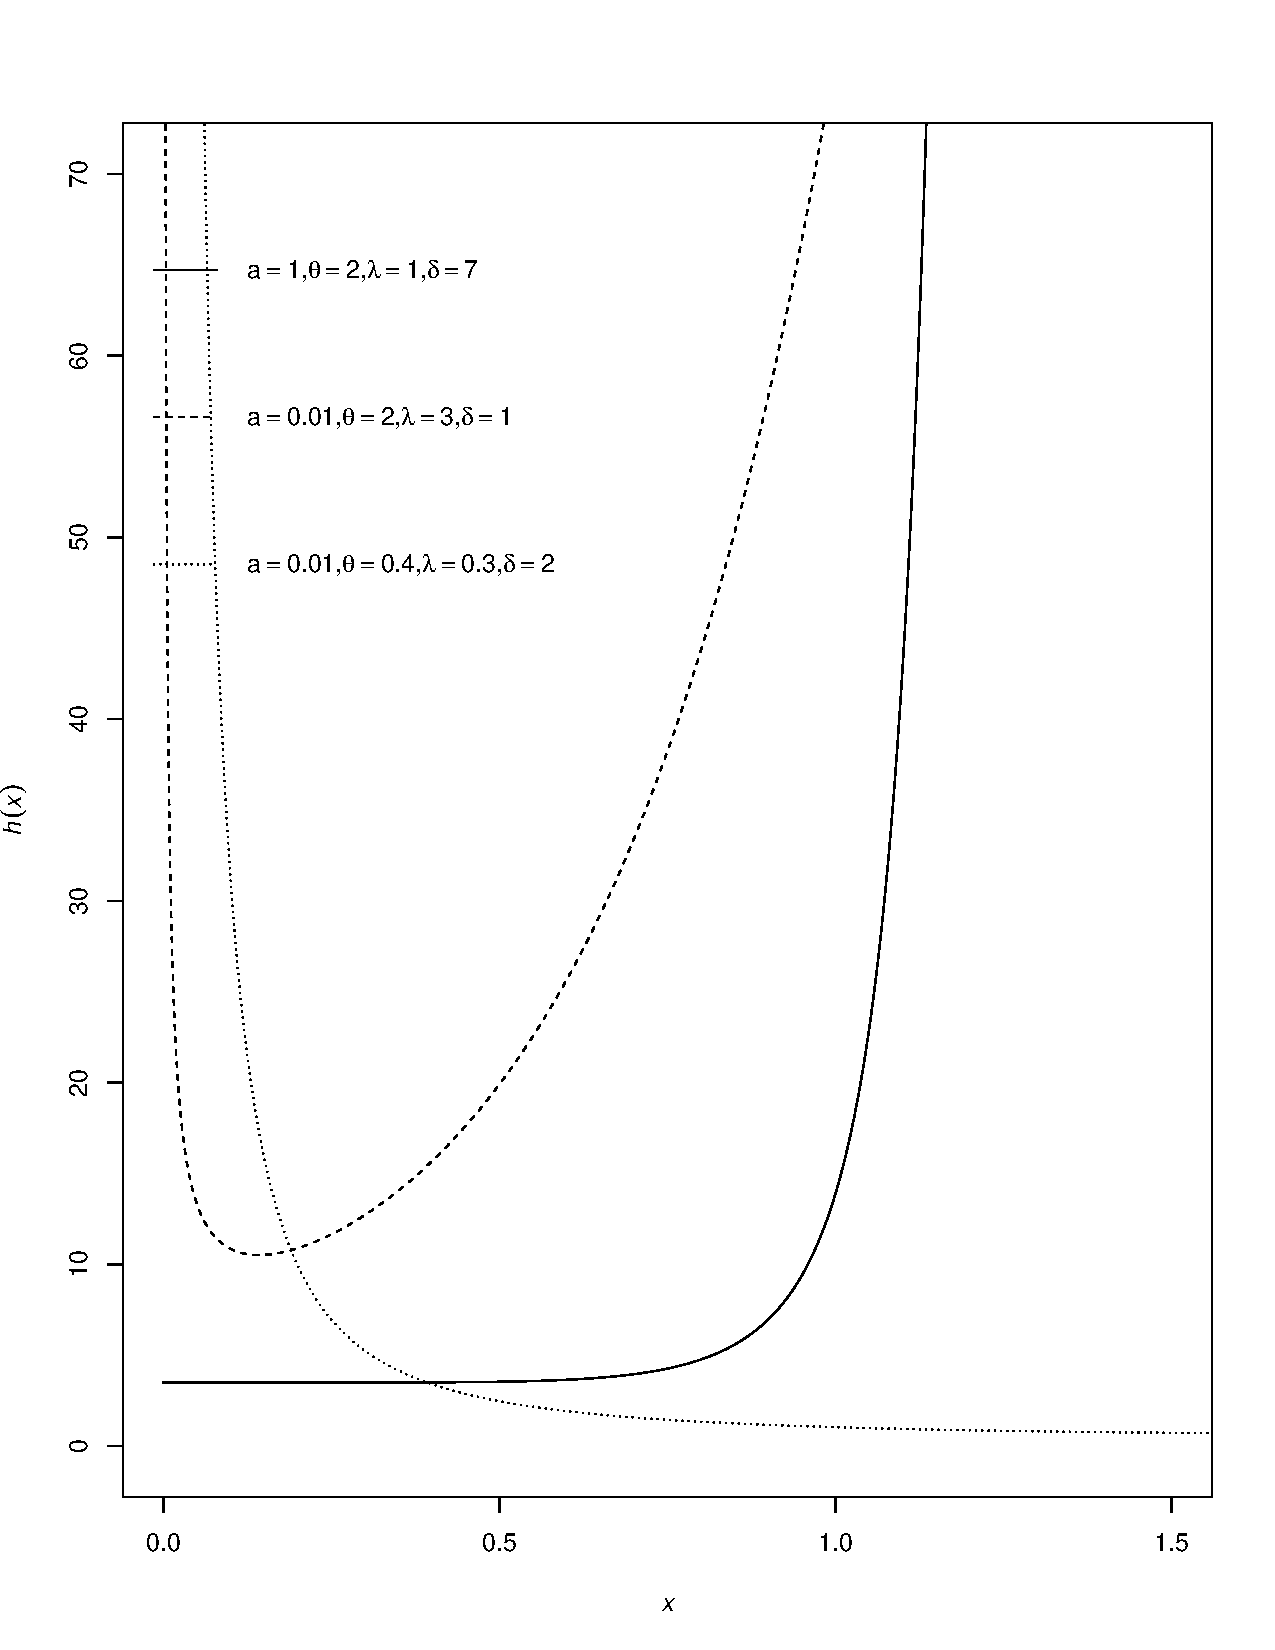
\includegraphics[scale=.3]{hazard.pdf}\\
%\vspace{-0.5cm}
%\caption{(a) Curves for the MO-$\Gamma$-W density; (b) Curves for the MO-$\Gamma$-W hazard;\label{formas}}
%\end{center}
%\end{figure}

\begin{landscape}
\begin{table}[htbp]\label{tabspecial1}
\centering
\begin{tabular}{c|c|c}
\hline
\textbf{Distribution} & \textbf{Baseline CDF} & \textbf{Generated PDF}  \\
\hline
{} & {} & {} \\
\textbf{Normal} &  $G(x)=\Phi(x)$ & $f_{X}(x)=\frac{\theta  \left\{ -\log[1-\Phi(x)] \right\}^{a-1}\, \phi(x)}{\Gamma(a)\,\left\{\theta+(1-\theta)\gamma_1\left( a, -\log \left[1-\Phi(x)\right]\right)\right\}^{2}}$ \\
{} & {} & {} \\
\hline
{} & {} & {} \\
\textbf{Logistic} &  $G(x)=\frac{1}{1+\rm{e}^{-x}}$ & $f_{X}(x)=\frac{\theta\,\rm{e}^{-x}\, \left\{ -\log[1-(1+\rm{e}^{-x})^{-1}] \right\}^{a-1}}{\Gamma(a)\,(1+\rm{e}^{-x})^{2}\,\left\{\theta+(1-\theta)\gamma_1\left( a, -\log \left[1-(1+\rm{e}^{-x})^{-1}\right]\right)\right\}^{2}}$\\
{} & {} & {} \\
\hline
\textbf{Gumbel} &  $G(x)=1-\exp(-\rm{e}^x)$ & $f_{X}(x)=\frac{\theta \, \exp(a \,x-  \rm{e}^x)}{\Gamma(a)\,\left\{\theta+(1-\theta)\gamma_1\left(a, \rm{e}^{x}\right)\right\}^{2}}$ \\
{} & {} & {} \\
\hline
{} & {} & {} \\
\textbf{Log-Normal} &  $G(x)=\Phi(\log x)$ & $f_{X}(x)=\frac{\theta\,\phi(\log x)\,  \left\{ -\log[1-\Phi(\log x)] \right\}^{a-1}}{\Gamma(a)\,x\,\left\{\theta+(1-\theta)\gamma_1\left( a, -\log \left[1-\Phi(\log x)\right]\right)\right\}^{2}}$ \\
{} & {} & {} \\
\hline
{} & {} & {} \\
\textbf{Exponential} &  $G(x)=1-\exp(-\lambda x),\,\lambda>0$ & $f_{X}(x)=\frac{\theta\,\lambda^{a}\,x^{(a-1)}\, }{\Gamma(a)\,\left\{\theta+(1-\theta)\gamma_1\left(a,\lambda x\right)\right\}^{2}}$ \\
{} & {} & {} \\
\hline
{} & {} & {} \\
\textbf{Weibull} &  $G(x)=1-\exp(-(\lambda x)^\gamma),\,\lambda,\gamma>0$ & $f_X(x)=\frac{\theta\,\gamma\lambda^{a\,\gamma}x^{a\,\gamma-1}\exp\{-(\lambda\,\gamma)^\gamma\}}{\Gamma (a)\{\theta+(1-\theta)\gamma_1[a,(\lambda\,x)^\gamma]\}^2}$ \\
{} & {} & {} \\
\hline
{} & {} & {} \\
\textbf{Gamma} &  $G(x)=\gamma_1(\alpha,\beta x),\,\alpha,\,\beta>0$ & $f_{X}(x)=\frac{\theta\,\beta^{\alpha}\,x^{\alpha-1}\,\rm{e}^{-\beta x}\,\left\{ -\log[1-\gamma_1(\alpha,\beta x)] \right\}^{a-1}}{\Gamma(a)\,\left\{\theta+(1-\theta)\gamma_1\left( a, -\log \left[1-\gamma_1(\alpha,\beta x)\right]\right)\right\}^{2}}$ \\
{} & {} & {} \\                                                                                                                                                                                                                                                                           \hline
\textbf{Pareto} &  $G(x)=1-\frac{1}{(1+x)^\nu},\,\nu>0$ & $f_{X}(x)=\frac{\theta \, \rm{e}^{-x}\, \left[\nu\log(1+x)\right]^{a-1}\, g(x)}{\Gamma(a)\,(1+\rm{e}^{-x})^2\,\left\{\theta+(1-\theta)\gamma_1\left( a, \nu\log[1+x]\right)\right\}^{2}}$\\
{} & {} & {} \\
\hline
{} & {} & {} \\
\hline
\end{tabular}
\caption{Special Distributions in the  MO-$\Gamma$-G family.}
\end{table}
\end{landscape}


The CDF \eqref{CDF_MO-Gamma-G} can be easily inverted to calculate the QF of the MO-$\Gamma$-G distribution,
say $x=Q_{X}(u)=F_X^{-1}(u)$ for $u \in (0,10$, in terms of the baseline QF $Q_G(\cdot)$. The inverse of
$F_{X}(x)=u$, where $u$ is a uniform number in $(0,1)$ is easily obtained. By combining the inverses
of Equations (\ref{CDF_MO})and \eqref{CDF_MO-Gamma-G}, $F_{X}(x)=u$ leads to
$z=z(u)=\theta u/[1-(1-\theta)u]$ and $\gamma_{1}\left(a, -\log[1-G(x)]\right)=z(u)$.
Then, the QF of $X$ can be expressed as
$$x=Q_G\left(v(u)\right),$$
where
$$v(u)=1-\exp\left[-\gamma_1^{-1}\big(a,z(u)\big)\right],$$
and $\gamma_1^{-1}(a,w)=Q^{-1}(a,1-w)$ is the inverse function of $\gamma_1(a,w)$. Some formulae for
$Q^{-1}(a,1-w)$ are given in http:// functions.wolfram.com/ GammaBetaErf/ InverseGammaRegularized/.




\section{Estimation}\label{estimation}

The  MO-$\Gamma$-G family can be  fitted to real data using the {\it AdequacyModel} package in the {\sf R} software.
This packa\-ge does not require to define the log-likelihood function and it computes the MLEs, their standard errors (SEs)
and the formal statistics defined in Section \ref{applications}. It is necessary to provide the
PDF and CDF of the distribution to be fitted to a data set.

For example, if $x_i$ is one observation from (\ref{PDF_MO-Gamma-G}) and $\etn$ is a $q$-parameter vector specifying $G(\cdot)$,
the log-likelihood function for $\boldsymbol{\theta}^\top=(a,\theta,\etn^\top)$ from $n$ observations is
\begin{align}\label{loglik}
\ell (\boldsymbol{\theta})=&\,n\log (\theta)+n\log(\gamma)+n\, a\, \gamma \log(\lambda)+(a\gamma-1)\sum_{i=1}^n{\log(x_i)}-\lambda^\gamma\sum_{i=1}^n{\log(x_i)}\nonumber \\ &
-n\log[\Gamma(a)]-2\sum_{i=1}^n{\log\{\theta+(1-\theta)\gamma_1[a,(\lambda\,x_i)^\gamma]\}}.
\end{align}

The {\it AdequacyModel} package to maximize (\ref{loglik}) uses the PSO (particle swarm optimization)
approach from the quasi-Newton BFGS, Nelder-Mead and simulated-annealing methods to maximize the log-likelihood function and it does not require
initial values. More details are available at {\tt https://rdrr.io/cran/AdequacyModel/}.


\section{Simulations}\label{sec:simulation}

Due to the probable absence of MLEs in closed-form for distributions belonging to the MO-$\Gamma $-G family, it is necessary to examine the
precision of the estimates calculated numerically. For doing that, the biases of the estimators of the parameters of the
MO-$\Gamma$-Dagum($\theta$, $a$, $\alpha$, $\beta$, $p$) distribution are determined, where $G\sim \mathrm {Dagum} (\alpha, \beta, p)$
is the baseline distribution. All parameters are taken equal to one for different sample sizes reported in Table \ref{tab:bias}.

Ten thousand Monte Carlo simulations are performed for each sample size to examine the numerical estimates calculated by the
BFGS method. The figures in Table \ref{tab:bias} indicate that this method behaves well when the sample size increases.
This is theoretically expected. However, in practice, difficulties can be faced in other families of distributions
due to the flatness of the log-likelihood function.

All simulations can be reproduced using the script in Appendix \ref{ap:simulation}. The simulations are parallelized and able to use all threads
available by a multicore processor, thus making them more computationally efficient and consequently requiring less time to complete.
The simulations are performed on a computer with an Intel Core i5-8265U processor with 8 threads working at a maximum frequency of 3.90 GHz,
requiring, on these hardware, a time of 14.36 hours to perform all simulations. The figures in Table \ref{tab:bias} reveal that the average
biases of the MLEs could be very reduced only for $n> 2,000$.

\begin{table}[H]
	\centering
	\caption{Average biases of the MLEs obtained using the BFGS method.}\label{tab:bias}
	\begin{tabular}{rrrrrrr}
		\hline
		$n$ & $B(\hat{\theta})$ & $B(\hat{a})$ & $B(\hat{\alpha})$ & $B(\hat{\beta})$ & $B(\hat{p})$ & \textbf{Time (mins)}\\
		\hline
		10 & 0.2376 & 2.1635 & 2.7557 & 1.6282 & 1.3057 & 1.1430\\
		20 & 0.4154 & 2.4639 & 1.5728 & 1.8082 & 0.7383 & 1.6248\\
		60 & 0.7214 & 2.2432 & 0.5667 & 1.8815 & 0.2872 & 3.3954\\
		100 & 0.6146 & 1.9579 & 0.3253 & 1.6148 & 0.2651 & 4.9628\\
		200 & 0.3838 & 1.3894 & 0.1827 & 1.1773 & 0.3701 & 8.1457\\
		400 & 0.2166 & 0.9635 & 0.1076 & 0.6181 & 0.3957 & 13.7370\\
		600 & 0.1269 & 0.7242 & 0.0772 & 0.3968 & 0.3637 & 17.9310\\
		1,000 & 0.0553 & 0.4885 & 0.0521 & 0.2328 & 0.2636 & 22.8784 \\
		2,000  &  0.0456 & 0.3087 &  0.0334 &  0.0990 & 0.1722 &  38.4593\\
		5,000 & -0.0058 & 0.1307 & 0.0146 & 0.0117 & 0.0171 & 52.8098\\
		10,000 & -0.0146 & 0.0842 & 0.0095 & 0.0095 & 0.0031 & 95.8380\\
		20,000 & -0.0090 & 0.0330 & 0.0038 & 0.0005 & -0.0099 & 126.4260\\
		30,000 & -0.0028 & 0.0183 & 0.0012 & -0.0036 & -0.0029 & 182.0760\\
		50,000 & -0.0057 & 0.0124 & 0.0015 & 0.0016 & -0.0021 & 291.9300\\
		\hline
	\end{tabular}
\end{table}

\section{Applications}\label{applications}

Consider the Weibull baseline. Two applications are provided to compare the new generated model with seven extended Weibull
distributions, namely the beta-Weibull ($\beta$-W) (Famoye {\it et al.}, 2005), Kumaraswamy Weibull (Kw-W) (Cordeiro and Nadarajah, 2010),
Marshall-Olkin Weibull (MO-W) (Ahmed {\it et al.}, 2017), Marshall-Olkin Extended Weibull (MOE-W) (Cordeiro {\it et al.}, 2019),
exponentiated Weibull (exp-W) (Mudholkar and Srivastava, 1993), gamma Weibull ($\Gamma$-W) Cordeiro {\it et al.}, 2016) and exponentiated
generalized Weibull (EG-W) (Oguntunde {\it et al.}, 2015) (with $a=1$). Some of these distributions are widely used in practice.

The log-likelihood for the Marshall-Olkin-Gamma-Weibull (MO-$\Gamma$-W) from one observation is
\begin{align}
\ell (\boldsymbol{\theta})=& \log (\theta)+\log (\gamma)+(a\,\gamma)\log (\lambda)+(a\,\gamma-1)\log(x)-(\gamma\, x)^\gamma-\log[\Gamma(a)]\nonumber \\ &-2\log\{\theta+(1-\theta)\gamma_1[a,(\lambda\,x)^\gamma]\},
\end{align}
where $\boldsymbol{\theta}=(a,\theta,\lambda,\gamma)^\top$. The components of the score function are

\begin{equation*}
U_{a}(\boldsymbol{\theta})=\gamma  \log (\lambda )+\gamma  \log (x)-\psi ^{(0)}(a)-\frac{2\left\{(1-\theta ) A-(1-\theta ) \psi ^{(0)}(a) \gamma_1 \left[a,(x \lambda
   )^{\gamma }\right]\right\}}{\theta\,\Gamma(a)+(1-\theta)\gamma_1\left[a,(x \lambda
   )^{\gamma }\right]},
\end{equation*}

\begin{equation*}
U_{\theta}(\boldsymbol{\theta})=\frac{1}{\theta}-\frac{2\left\{\Gamma(a)-\gamma_1\left[a,(\lambda\,x)^\gamma\right]\right\}}{\theta\,\Gamma(a)+(1-\theta)\gamma_1\left[a,(\lambda\,x)^\gamma\right]},
\end{equation*}

\begin{equation*}
U_{\lambda}(\boldsymbol{\theta})=\frac{\gamma }{\lambda }\left[a-(\lambda\,x)^\gamma\right]+\frac{2 \gamma \,\lambda^{-1}(\lambda\,x)^{a\,\gamma} (1-\theta )\exp\{-(\lambda\,x)^\gamma\} }{\theta \,\Gamma(a)+(1-\theta )
   \gamma_1 \left[a,(x \lambda )^{\gamma }\right]}
\end{equation*}
and
\begin{equation*}		
U_{\gamma}\boldsymbol{\theta}=\frac{1}{\gamma }+a \log (\lambda )+a \log (x)-(\lambda  x)^{\gamma } \log
   (\lambda  x)+\frac{2 (1-\theta )(\lambda
   x)^{\gamma\,a } \log (\lambda  x)\exp\{-(\lambda  x)^{\gamma }\}  }{\theta \,\Gamma(a)+(1-\theta )
   \gamma_1 \left[a,(x \lambda )^{\gamma }\right]},
\end{equation*}
where
\begin{align*}
A=G_{2,3}^{3,0}\left[(x \lambda )^{\gamma }\Big{|}
\begin{array}{c}
 1,1 \\
 0,0,a \\
\end{array}
\right]+\log \left[(\lambda  x)^{\gamma }\right] \gamma_1 \left[a,(x \lambda )^{\gamma
   }\right],
\end{align*}
$\psi^{(n)}(x)$ is the $n$-th derivative of the digamma function,
\begin{eqnarray*}
A=\psi^{(0)}(a) - \log\left[(\lambda x)^{\gamma}\right]-G^{3,0}_{2,3}\,\left((\lambda x)^{\gamma} \Big{|}	\stackrel{1,1}{0,0,a}\right),
\end{eqnarray*}
and $G^{m,n}_{p,q}\,\left(z \Big{|}	\stackrel{a_{1},\ldots,a_{p}}{b_{1},\ldots,b_{q}}\right)$ is the Meijer G function.

The {\it AdequacyModel} package is used to fit the distributions cited before to two real data sets. The SANN method, which is a
variant of simulated annealing (Belisle, 1992), is considered. The distributions are compared via the Anderson
Darling (A$^{*}$) and Cram\'er Von Mises (W$^{*}$) statistics reported in the {\it goodness.fit} function.

For the first data set, a modification of the ``FoodExpenditure'' data from the {\it betareg} package in {\sf R} software is considered, which refers
to the proportions of income spent on food for a random sample of 38 households in a large US city (according to the package information).
Here, the household expenditures for food are considered and is given by
\begin{eqnarray*}
data = FoodExpenditure_{food} / \#(FoodExpenditure_{food}),
\end{eqnarray*}
where $FoodExpenditure_{food}$ is the random variable corresponding to the household expenditures for food and $\#(\cdot)$ indicates the number of
observations on this variable. The MLEs and their standard errors (SEs) (in parentheses) are listed in Table \ref{tab-ex1}.
The statistics  W$^{*}$ and A$^{*}$ are also given in this table. The results indicate that the proposed model has better performance than the other
seven fitted models.


\begin{table}[!htb]
\scriptsize
\center
\caption{  \small Application 1}
\label{tab-ex1}
\begin{tabular}{lcccccc}
\hline\noalign{\smallskip}
Model & $a$ & $\theta$ & $\lambda$ & $\gamma$ &  $W^*$ & $A^*$   \\
\hline \\
 & & & & &  \\
MO-$\Gamma$-W$(a,\theta,\lambda,\gamma)$    &  0.926134 & 1.379664 & 33.323073 & 25.398809 & 0.0339 &  0.2376 \\                            &    (0.02626926) & (0.22381086) & (0.28530971) & (0.08259864)  & & \\

 & & & & &  \\
$\beta-$W$(a,\theta,\lambda,\gamma)$ &   9.92882 &  0.1700880 & 9.759469 & 1.530541  & 0.043567 & 0.2594618\\
                                    &    (0.02908181) & (0.02049663) & ($<$0.0001) & ($<$0.0001)  && \\
                                                                                & & & & &  \\
KW-W$(a,\theta,\lambda,\gamma)$ &    0.04987575 & 99.99989793 &  1.07602954 & 23.40287099 & 1.330915 & 6.742609\\
                                       &    (0.008090352) & (16.225905058) &  (0.003156126) &  (0.014646102) && \\																						 & & & & &  \\
                                       MOE-W$(a,\theta,\lambda,\gamma)$  &  0.1366666 & 2.020436 & 62.72201 & 4.2956659  &0.03541554 & 0.2579222 \\
 & (0.1599182) & ($<$0.0001) &($<$0.0001) & (0.7365535)    &  & \\
                                                                              & & & & &  \\
EGW$(a,b,\lambda,\gamma)$    &  5.6189861421 &  6.1833138579 &  1.2870816760  & 1.3798562942  &  0.03715255 & 0.2518879 \\
& (0.0028147823) & (0.0009807091) & (0.1159810838) & (0.1480747352)    &  & \\
                                                           & & & & &  \\                                                           MO-W$(a,\lambda,\gamma)$  & 0.15920715  & - &  1.58609458  & 4.26713785  &  0.03456333   & 0.257339\\
&    (0.07170351) & (-) & (0.13353716) & (0.16650667)  &  & \\

 & & & & &  \\
exp-W$(a,\lambda,\gamma)$   &    6.1102948   & - &   4.4680469 &  1.3858740 &   0.03726684   & 0.2523749 \\
&   (0.4222173) & (-) & (0.3175876) & (0.1677722)   &  & \\

 & & & & &  \\
$\gamma$-W$(a,\lambda,\gamma)$    & 5.751546  & - &  10.0000 & 1.208773&  0.0879 & 0.6599  \\
&  (0.0015006)&  (-)&  (0.0001163185) &(0.00822782)    &  & \\

 & & & & &  \\





%GammaBS$(a,b,\alpha)$     &  1.2354 & 40.4438 &  0.1379 &       & 0.4931 &   2.7656 &  0.3725 & $1.765x10^{-12}$\\
                          %&  ( 0.0025)& ( 14.6913)& (0.0446) &      & &&  && \\
                                                     \hline
\end{tabular}
\end{table}



As a second application, consider a data set collected in a pilot study about hypertension in the Dominican Republic
in 1997 found in http://biostat.mc.vanderbilt.edu/wiki/
Main/DataSets. The observations are the systolic blood pressure of persons who came to medical clinics in
several villages for a variety of complaints. The MLEs of the parameters, their SEs and the values of the statistics are
listed in Table \ref{tab-ex2} for the previous distributions. By comparing the measures of these formal statistics,
we conclude that the proposed distribution outperforms the rest of them.

\begin{table}[htb!]
\scriptsize
\center
\caption{  \small Application 2}
\label{tab-ex2}
\begin{tabular}{lcccccc}
\hline\noalign{\smallskip}
Model & $a$ & $\theta$ & $\lambda$ & $\gamma$ &  $W^*$ & $A^*$   \\
\hline
 & & & & &  \\
MO-$\Gamma$-W$(a,\theta,\lambda,\gamma)$    &  9.629304 & 3.640779 & 6.260826 & 12.823429 &0.5093&  2.8076 \\
                                       &    (0.006217876) & (0.182495785) & (0.024446563) & (0.007965221)  && \\

 & & & & &  \\
 $\beta-$W$(a,\theta,\lambda,\gamma)$ &   31.08471 &  47.14636 &   0.01698383 &  2.054037 & 0.7540428 & 4.279418\\
&    (0.01279570) & ($<$0.0001) & (0.00014535) & ($<$0.0001)  && \\

 & & & & &  \\
KW-W$(a,\theta,\lambda,\gamma)$ &   7363.281 & 0.03925762 &  1.467640 &   0.6146940 & 0.5351 & 2.9617\\
                                       &    (0.04194304) & (0.0004194304)& ($<$0.0001)& ($<$0.0001) && \\

 & & & & &  \\
 MOE-W$(a,\theta,\lambda,\gamma)$  &  101.13471834 &  0.42386507  & 0.03095935 &  1.70240332  &1.14418 & 6.644617 \\
                            & (46.782882038) &  (0.100832102) &  (0.003644092) &  (0.168142275)   &  & \\

 & & & & &  \\
 EGW$(a,b,\lambda,\gamma)$    &  0.2351691 &  140.0000 &   0.4576370 &   0.7425738 &  0.8925 & 5.3338 \\
                            & (0.002540837) & (3.278565) & ($<$0.0001) & ($<$0.0001)   &  & \\

 & & & & &  \\
 MO-W$(a,\lambda,\gamma)$  & 173.2139  & - &  0.02125455 &  1.601970  &  1.476088   & 8.58705\\
                                       &    (0.00016394) & (-) & (0.000212794) & (0.0001398109)  &  & \\

 & & & & &  \\
 exp-W$(a,\lambda,\gamma)$   &    69.02916  & - &   0.02405120 & 1.345536 &   0.8899261   & 5.094141 \\
                          &   (0.08389090) & (-) & (0.0002249256) & ($<$0.0001)   &  & \\

 & & & & &  \\
 $\Gamma$-W$(a,\lambda,\gamma)$    & 9.11229459   & - &  0.02617729 & 1.74641178 &    0.6227098 & 3.488268  \\
                             &  (0.96330688)&  (-)&  (0.00291875) & (0.08030313)     &  & \\

 & & & & &  \\




%GammaBS$(a,b,\alpha)$     &  1.2354 & 40.4438 &  0.1379 &       & 0.4931 &   2.7656 &  0.3725 & $1.765x10^{-12}$\\
                          %&  ( 0.0025)& ( 14.6913)& (0.0446) &      & &&  && \\
                                                    \hline
\end{tabular}
\end{table}





\section{Mathematical properties}\label{properties}


In this section, some main mathematical properties are presented for the MO-$\Gamma$-G family
based on a general linear representation for its density function, which are important
to determine its mathematical properties from those of exponentiated-G (exp-G) distributions.

\subsection{Linear Representation}


For an arbitrary CDF $G(x)$, the CDF and PDF of the exponentiated-G (exp-G) distribution with power parameter $a>0$ are
\begin{eqnarray*}
\Pi_a(x)=G(x)^a\qquad\text{and}\qquad\pi_a(x)=a\,g(x)\,G(x)^{a-1},
\end{eqnarray*}
respectively. This class of distributions is quite useful in several applications. In fact, Tahir and Nadarajah (2015)
cited more than seventy papers on exponentiated distributions in their Table 1.

First, the MO-G cumulative distriution (\ref{densityMO}) admits the
linear combination (Barreto-Souza \emph{et al.}, 2013)
\begin{equation}
F_{\text{MO}-\Gamma}(x)
\,=\,
\sum^{\infty}_{i=0}\,w_i^{\text{MO-G}}\,\Pi_{i+1}(x)\,=\,\sum^{\infty}_{i=0}\,w_i^{\text{MO-G}}\,G(x)^{i+1},
\label{EXP44}
\end{equation}
where the coefficients are (for $i=0,1,\ldots$)
\[
w_i^{\text{MO}-\Gamma}=w_i^{\text{MO}-\Gamma}(\theta) =
\begin{cases}
\dfrac{(-1)^i\,\theta}{(i+1)} \sum\limits^{\infty}_{j=i}(j+1)\,\dbinom{j}{i}\,\bar{\theta}^j,& \quad \theta\in (0,1),\\
\theta^{-1} (1-\theta^{-1})^i,& \quad \theta>1,
\end{cases}
\]
and $\bar{\theta}=1-\theta$.


Second, the linear combination for the $\Gamma\text{-G}$ cumulative distribution (\ref{PDF_Ga}) follows from Castellares and Lemonte (2015) as
\begin{equation}\label{EXP33}
F_{\Gamma\text{-G}}(x)\,=\,\sum_{j=0}^\infty w_{j}^{\Gamma\text{-G}}\,\,\Pi_{a+j}(x).
\end{equation}
Here,
$$w_j^{\Gamma\text{-G}}=w_j^{\Gamma\text{-G}}(a)=\frac{\varphi_{j}(a)}{(a+j)},$$
\begin{equation*}\label{coeficientes}
\varphi_0(a)=\frac{1}{\Gamma(a)},
\quad\,
\varphi_j(a)=\frac{(a-1)}{\Gamma(a)}\,\psi_{j-1}(j+a-2),\quad j\geq 1,
\end{equation*}
and
\begin{align*}\label{polinomios_ward}
\begin{split}
\psi_{n-1}(x)&=\frac{(-1)^{n-1}}{(n+1)!}\Biggl[H^{n-1}_{n}-\frac{x+2}{n+2}H^{n-2}_{n}
+ \frac{(x+2)(x+3)}{(n+2)(n+3)}H^{n-3}_{n}- \cdots\\
&\qquad+ (-1)^{n-1}\frac{(x+2)(x+3)\cdots(x+n)}{(n+2)(n+3)\cdots(2n)}H^{0}_{n}\Biggr],
\end{split}
\end{align*}
is the Stirling polynomial, $H^{m}_{n+1}=(2n+1-m)H^{m}_{n} + (n-m+1)H^{m-1}_{n}$ is a positive integer,
$H^0_0=1$, $H^{0}_{n+1}=1\times 3\times 5\times\cdots\times(2n+1)$ and $H^{n}_{n+1}=1$.

By inserting \eqref{EXP33} in Equation \eqref{EXP44} and via a result for a power series raised to a positive integer (Gradshteyn and
Ryzhik, 2000), the expansion for the cdf of the MO-$\Gamma$-G distribution reduces to
\begin{align*}
F_{\text{MO}-\Gamma\text{-G}}(x)&=\sum_{i=0}^{\infty}\,w_{i}^{\text{MO-}\Gamma}\,G(x)^{(i+1)a}\,\left[\sum_{j=0}^{\infty}\,w_{j}^{\Gamma\text{-G}}\,G(x)^{j}\right]^{i+1}\\
&=\sum_{i=0}^{\infty}\,w_{i}^{\text{MO-}\Gamma}\,G(x)^{(i+1)a}\,\sum_{j=0}^{\infty}\,c_{i+1,j}\,G(x)^{j} =\sum_{i,j=0}^\infty d_{i,j}\,\Pi_{(i+1)a+j}(x),
\end{align*}
where $d_{i,j}=d_{i,j}(a,\theta)=w_{i}^{\text{MO-G}}\,c_{i+1,j}(a)$, $c_{i+1,0}(a)=(w_{0}^{\Gamma\text{-G}})^{i+1}$ and, for $m \ge 1$,
$c_{i+1,m}(a)=\frac{1}{m w_{0}^{\Gamma\text{-G}}}\,\sum^{m}_{r=1}\,\left[r(i+2)-m\right]\,w_{r}^{\Gamma\text{-G}}\,c_{i+1,m-r}(a)$.

By differentiating the last equation, the expansion for the MO-$\Gamma$-G density follows as
\begin{equation}\label{lcom}
f_{\text{MO}-\Gamma\text{-G}}(x)=\sum_{i,j=0}^\infty d_{i,j}\,\pi_{(i+1)a+j}(x).
\end{equation}

So, some structural properties of the proposed family can be determined from the double linear combination (\ref{lcom})
and those properties of the exp-G distribution. In most applications, the indices $i$ and $j$ can vary up to five.


\subsection{Some quantities}

Hereafter, let $T_{i,j}\sim$exp-G$[(i+1)a+j]$. The $n$th moment of $X$ can be obtained from (\ref{lcom}) as
\begin{eqnarray}\label{moment}
\displaystyle
\mu_n^{\prime}=E(X^n)=\sum_{i,j=0}^\infty d_{i,j}\,E(T_{i,j})=\sum_{i,j=0}^\infty \,[(i+1)a+j-1]\,d_{i,j}\,\tau[n,(i+1)a+j-1],
\end{eqnarray}
where
\begin{eqnarray*}
\tau(n,a)=\int_{-\infty}^{\infty} x^n\,G(x)^{a}\,g(x)dx=\int_{0}^{1} Q_G(u)^n\,u^a d u.
\end{eqnarray*}

Expressions for moments of several exponentiated distributions can be found in the papers
cited in Tahir and Nadarajah (2015, Table 1). We give just one example from Equation (\ref{moment})
by taking the exponential distribution with rate $\lambda>0$ for the baseline G.
It follows easily as
\begin{eqnarray*}
\mu_n^{\prime}= n!\,\lambda^n\,\sum_{i,j,m=0}^\infty \,\frac{(-1)^{n+m}\,[(i+1)a+j]\,d_{i,j}}{(m+1)^{n+1}}\,\binom{(i+1)a+j-1}{m}.
\end{eqnarray*}

A general expansion for the moment generating function (MGF) $M(t)=E(\rm{e}^{t\,X})$ of $X$ can be expressed from (\ref{lcom})
\begin{eqnarray}\label{mgf}
\displaystyle
M(t)=\sum_{i,j=0}^{\infty} \,d_{i,j}\,M_{i,j}(t)=\sum_{i,j=0}^{\infty}\, [(i+1)a+j]\,d_{i,j}\,\rho(t,(i+1)a+j-1),
\end{eqnarray}
where $M_{i,j}(t)$ is the MGF of $Y_{i,j}$ and
\begin{eqnarray*}
\rho(t,a)=\int_{-\infty}^{\infty}\,\rm{e}^{t x}\,G(x)^{a}\,g(x) dx=\int_{0}^{1}\exp\left\{t\,Q_G(u)\right\}\,u^a d u.
\end{eqnarray*}

The MGFs of many MO-$\Gamma$-G distributions can be determined from Equation (\ref{mgf}).
For example, the generating function of the MO-$\Gamma$-exponential with parameter $\lambda$
(if $t<\lambda^{-1}$) is
\begin{eqnarray*}
\displaystyle
M(t)=\sum_{i,j=0}^{\infty} [(i+1)a+j]\,d_{i,j}\,\,B((i+1)a+j,1-\lambda t).
\end{eqnarray*}

For empirical purposes, the shape of many distributions can be usefully described by
the incomplete moments. These moments play an important role for measuring
inequa\-lity. For example, the mean deviations and Lorenz and Bonferroni curves depend upon the first incomplete moment of the distribution.
The $n$th incomplete moment of $X$ can be expressed as
{\small
\begin{eqnarray}\label{incomplete}
\displaystyle
\qquad
m_{n}(y)=\int_{-\infty}^y x^n\,f_{X}(x) dx = \sum_{i,j=0}^{\infty} [(i+1)a+j]\,d_{i,j}\,\int_{0}^{G(y)}\,Q_G(u)^n\, u^{(i+1)a+j-1}\,du.
\end{eqnarray}
}
The definite integral in (\ref{incomplete}) can be evaluated for most baseline G distributions.



\section{Conclusions}\label{conclusions}

A new family of distributions called the Marshall and Olkin-Gamma-G family with two shape parameters is introduced. The estimation of the unknown
parameters is done via the maximum likelihood method and a simulation study is conducted to verify its adequacy. Additionally, the usefulness
of the proposed family is shown empirically by means of two applications to real data.

\appendix

\section{Appendix: Simulation code}\label{ap:simulation}

The script below is used to perform the simulations whose results are given in Table \ref{tab:bias} of Section \ref{sec:simulation}.
It is developed a script using the programming language {\sf R} to be used in other simulations or even to check the results presented in this paper.


%\lstinputlisting[language=R, caption={Monte-Carlo simulations for different sample sizes.}, numbers=left,
%stepnumber=1,
%showspaces=false,
%tabsize=4,
%basicstyle=\scriptsize,
%backgroundcolor=\color{lbcolor},
%showstringspaces=false]{new_code_dagum.R}


\section*{References}

\begin{description}

\item
A. Alzaatreh, F. Famoye, C. Lee:
A new method for generating families of continuous distributions.
Metron {\bf 71}(1) 63-79 (2013).

\item
W. Barreto-Souza, A.J. Lemonte, G.M. Cordeiro:
General results for the Marshall and Olkin's family of distributions.
Anais da Academia Brasileira de Ci\^{e}ncias {\bf 85}(1) 3-21 (2013).

\item
Z.W. Birnbaum, S.C. Saunders:
A new family of life distributions.
Journal of Applied Probability {\bf 6}(2) 319-327 (1969).

\item
F. Castellares, A.J. Lemonte:
A new generalized Weibull distribution gene\-rated by gamma random variables.
Journal of the Egyptian Mathematical Society {\bf 23}(2) 382-390 (2015).

\item
G.M. Cordeiro, M. de Castro:
A new family of generalized distributions.
Journal of Statistical Computation and Simulation {\bf 81}(7) 883-898 (2011).

\item
N. Eugene, C. Lee, F. Famoye:
Beta-normal distribution and its applications.
Communications in Statistics -- Theory and Methods {\bf 31}(4) 497-512 (2002).

\item

Gradshteyn IS, Ryzhik IM: Table of Integrals, Series and Products. Sixth edition. San Diego: Academic Press (2000).

\item
R.C. Gupta, R.D. Gupta, P.L. Gupta:
Modeling failure time data by Lehmann alternatives.
Communications in Statistics -- Theory and Methods {\bf 27}(4) 887-904 (1998).

\item
R.D. Gupta, D. Kundu:
Exponentiated exponential family: an alternative to gamma and Weibull distributions.
Biometrical Journal {\bf 43}(1) 117-130 (2001).

%\item
%P. Kumaraswamy:
%Generalized probability density-function for double-bounded
%random-processes. Journal of Hydrology {\bf 46}(1-2) 79-88 (1980).

\item
A.J. Lemonte, G.M. Cordeiro, G. Moreno-Arenas:
A new useful three-parameter extension of the exponential distribution.
Statistics {\bf 50}(2) 312-337 (2016).

\item
A.W. Marshall, I. Olkin:
A new method for adding a parameter to a family of distributions with
application to the exponential and Weibull families.
Biometrika {\bf 84}(3) 641-652 (1997).

\item
G.S. Mudholkar, D.K. Srivastava:
The exponentiated Weibull family: a reanalysis of the bus-motor-failure data.
Technometrics {\bf 37}(4) 436-445 (1995).

\item
S. Nadarajah, G.M. Cordeiro, E.M.M. Ortega:
Some general results for the beta-modified Weibull distribution.
Journal of Statistical Computation and Simulation {\bf 81}(10) 1211-1232 (2011).

\item
S. Nadarajah, G.M. Cordeiro, E.M.M. Ortega:
General results for the Kumaraswamy G distribution.
Journal of Statistical Computation and Simulation {\bf 87}(7) 951-979 (2012).

\item
S. Nadarajah, A.K. Gupta:
The exponentiated gamma distribution with application to drought data.
Calcutta Statistical Association Bulletin {\bf 59}(1-2) 29-54 (2007).

\item
S. Nadarajah, F. Haghighi:
An extension of the exponential distribution.
Statistics {\bf 45}(6) 543-558 (2011).

\item
S. Nadarajah, S. Kotz:
The exponentiated-type distributions.
Acta Applicandae Mathematicae {\bf 92}(2) 97-111 (2006).

\item
M.D. Nichols, W.J. Padgett:
A Bootstrap control chart for Weibull percentiles.
Quality and Reliability Engineering International {\bf 22}(2) 141-151 (2006).

\item
F. Proschan:
Theoretical explanation of observed decreasing failure rate.
Technometrics {\bf 5}(3) 375-383 (1963).

\item
M.M. Risti\'{c}, N. Balakrishnan:
The gamma-exponentiated exponential distribution.
Journal of Statistical Computation and Simulation {\bf 82}(8) 1191-1206 (2012).

\item
E.W. Stacy: A Generalization of the Gamma Distribution. Annals of Mathematical Statistics {\bf 33}(3) 1187-1192 (1962).

\item
M.H. Tahir, S. Nadarajah:
Parameter induction in continuous univariate distributions: Well-established G families.
Anais da Academia Brasileira de Ci\^{e}ncias {\bf 87}(2) 539-568 (2015).

\item
K. Zografos, N. Balakrishnan:
On families of beta-and generalized gamma-generated distribution and
associate inference.  Statistical Methodology {\bf 6}(4) 344-362 (2009).

\end{description}




\end{document}
